\documentclass{standalone}
% 
% polinomis creats amb el fitxer ../code/polinomisBeziers.mlx
\usepackage{pgfplots}

\usepackage{mathtools}
\pgfplotsset{compat=1.8}



\begin{document}

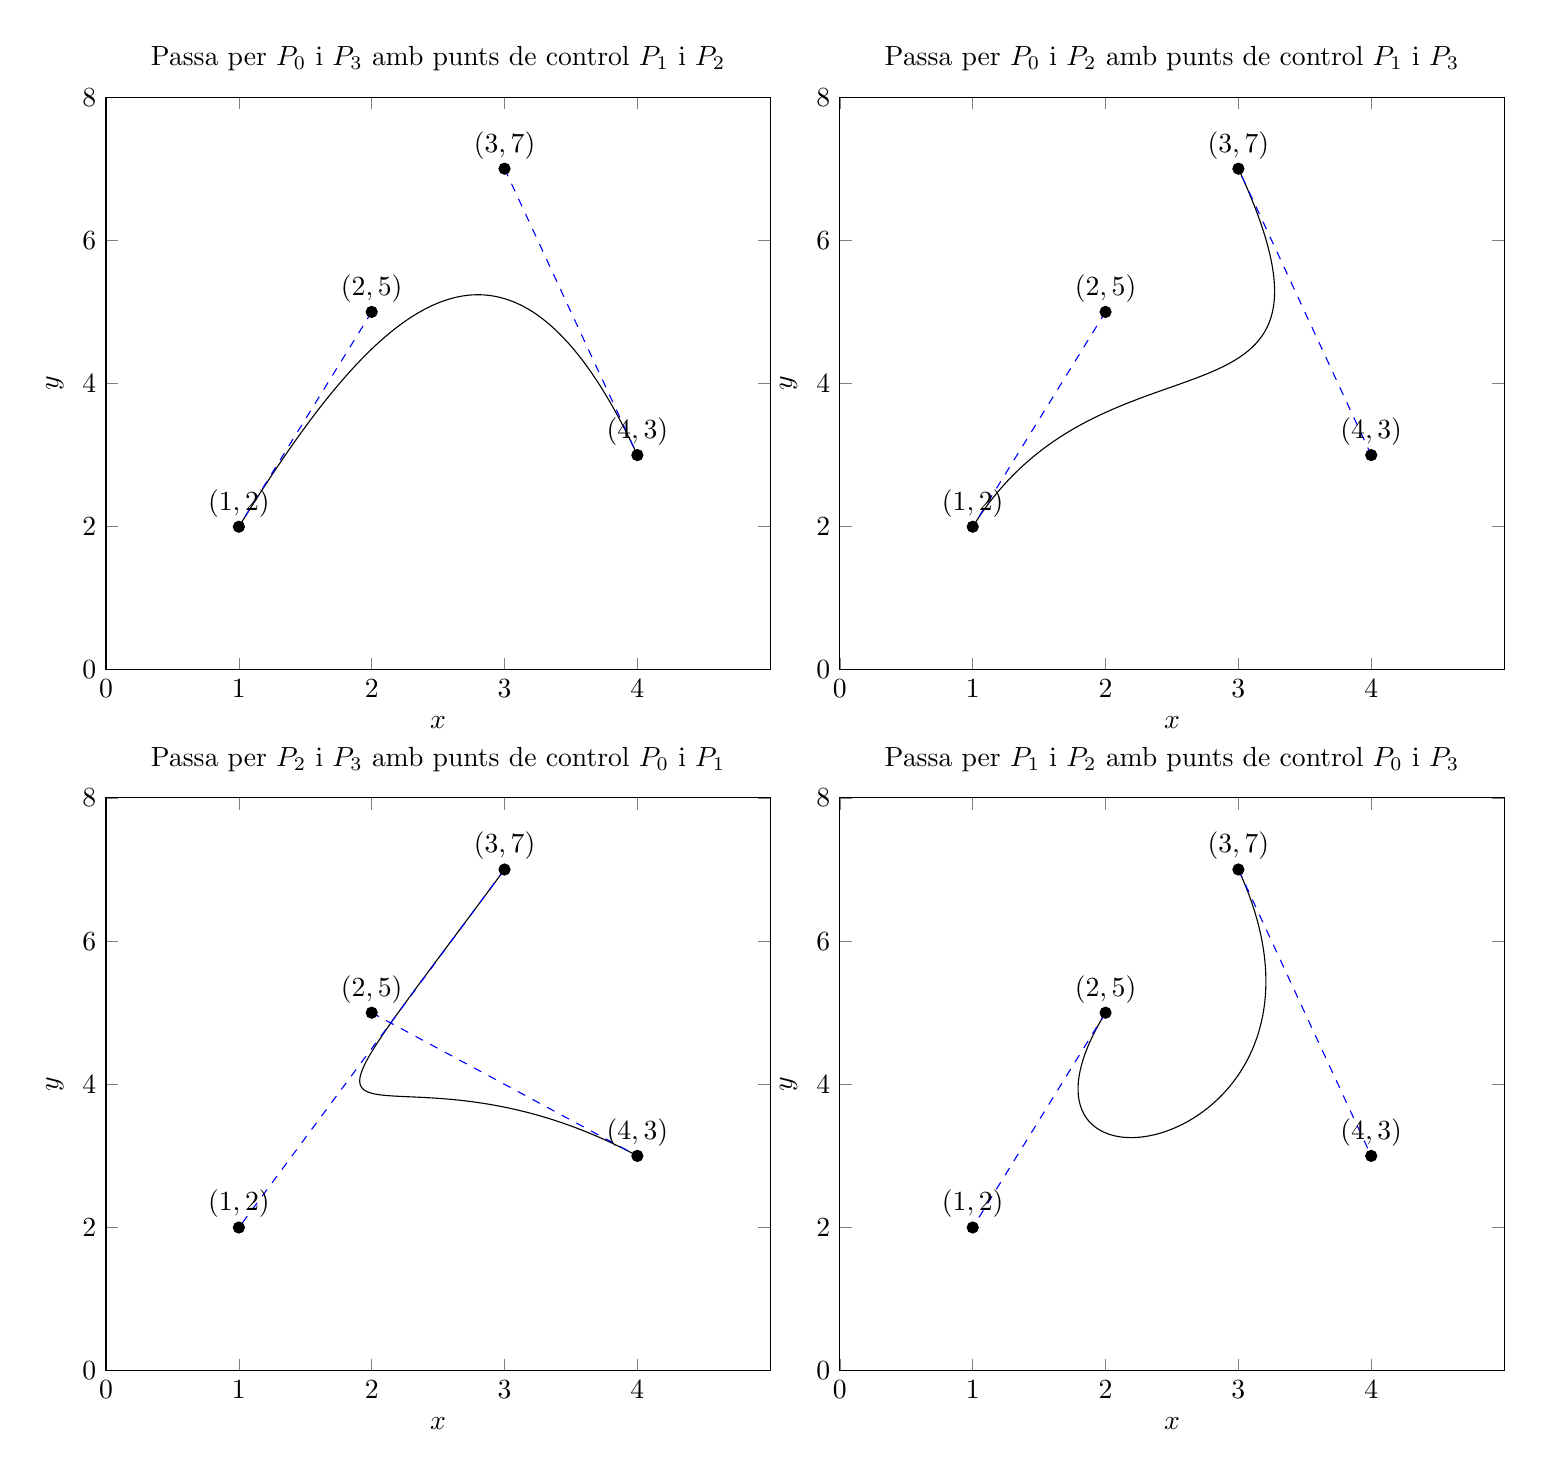
\begin{tikzpicture}
\pgfplotsset{
  scale only axis,
  xmin=0,xmax=5,
  ymin=0,ymax=8,
  xlabel=$x$,
  ylabel=$y$,
  samples=100,
  xtick={0,1,2,3,4}
%  yticklabel style={text width=3em,align=right}% important per mantenir una mida correcta dels ticks en qualsevol situació quan hi ha multiple plots
}

\matrix{

\begin{axis}[
  title={Passa per $P_0$ i $P_3$ amb punts de control $P_1$ i $P_2$},
  name=plot1,
  ]
  \addplot [only marks,mark=*,nodes near coords={$(\pgfmathprintnumber{\pgfkeysvalueof{/data point/x}},
  \pgfmathprintnumber{\pgfkeysvalueof{/data point/y}})$}]
  table {
   1 2
   2 5
   3 7
   4 3
   };
 \addplot[][domain=0:1]({3*x+1},{-5*x^3-3*x^2+9*x+2});
 \addplot[dashed,blue] coordinates {(3,7) (4,3)};
 \addplot[dashed,blue] coordinates {(2,5) (1,2)};
\end{axis}

&\begin{axis}[
  title={Passa per $P_0$ i $P_2$ amb punts de control $P_1$ i $P_3$},
  name=plot2,
  %at=(plot1.right of south east), anchor=left of south west,
  ]
  \addplot [only marks,mark=*,nodes near coords={$(\pgfmathprintnumber{\pgfkeysvalueof{/data point/x}},
   \pgfmathprintnumber{\pgfkeysvalueof{/data point/y}})$}]
   table {
    1 2
    2 5
    3 7
    4 3
    };
  \addplot[][domain=0:1]({-4*x^3+3*x^2+3*x+1},{11*x^3-15*x^2+9*x+2});
  \addplot[dashed,blue] coordinates {(4,3) (3,7)};
  \addplot[dashed,blue] coordinates {(2,5) (1,2)};
\end{axis}

\\
\begin{axis}[%
  title={Passa per $P_2$ i $P_3$ amb punts de control $P_0$ i $P_1$},
  name=plot4,
  %at=(plot1.below south west), anchor=above north west,
  ]
  \addplot [only marks,
            mark=*,
            nodes near coords={$(\pgfmathprintnumber{\pgfkeysvalueof{/data point/x}},
   \pgfmathprintnumber{\pgfkeysvalueof{/data point/y}})$}] table {
    1 2
    2 5
    3 7
    4 3
    };
    \addplot[][domain=0:1]({-2*x^3+9*x^2-6*x+3},{-13*x^3+24*x^2-15*x+7});
    \addplot[dashed,blue] coordinates {(2,5) (4,3)};
    \addplot[dashed,blue] coordinates {(3,7) (1,2)};
\end{axis}

&\begin{axis}[%
  title={Passa per $P_1$ i $P_2$ amb punts de control $P_0$ i $P_3$},
  name=plot3,
  %at=(plot2.below south west), anchor=above north west,
  ]
  \addplot [only marks,
              mark=*,
              nodes near coords={$(\pgfmathprintnumber{\pgfkeysvalueof{/data point/x}},
     \pgfmathprintnumber{\pgfkeysvalueof{/data point/y}})$}] table {
      1 2
      2 5
      3 7
      4 3
      };
      \addplot[][domain=0:1]({-8*x^3+12*x^2-3*x+2},{-x^3+12*x^2-9*x+5});
      \addplot[dashed,blue] coordinates {(2,5) (1,2)};
      \addplot[dashed,blue] coordinates {(3,7) (4,3)};
\end{axis}

\\
};

\end{tikzpicture}

\end{document}
